\documentclass[xcolor=table, aspectratio=169, bigger]{beamer}

\usepackage{shyne}

% Theme settings
\setbeamertemplate{navigation symbols}{}

\usetheme{Madrid}
\usefonttheme{structurebold}
\usefonttheme[onlymath]{serif}

\AtBeginSection[]
{ 	\begin{frame}{}

	{
	\usebeamerfont{frametitle}
	\begin{beamercolorbox}
		[wd={\textwidth}, center, sep=.2in, rounded=true, shadow=true]
		{frametitle}
	Week \thesection\\  \secname 
	\end{beamercolorbox}
	}
	
	\end{frame} 
}

\AtBeginSubsection[]
{ 	\begin{frame}{}

	{
	\usebeamerfont{frametitle}
	\begin{beamercolorbox}
		[wd={\textwidth}, center, sep=.2in, rounded=true, shadow=true]
		{frametitle}
	Section \thesection .\thesubsection\\  \subsecname 
	\end{beamercolorbox}
	}
	
	\end{frame} 
}

\title[Week 8]{Stat 201: Statistics I\\Week 10 }
\author[M. Shyne]{}
\institute[Metro State]{
\includegraphics[width=1.75in]{../images/metro_logo}}
\date[4/14/2019]{
\\ \bigskip \bigskip 
\includegraphics[width=.4in]{../images/cc_big}}



\begin{document}
\frame{\titlepage}

% Week 10
\setcounter{section}{9}
\section{Inference for Categorical Data}

%
% Section 10.1
%
\subsection{Hypothesis tests for proportions}

%%%%%%%%%%
\begin{frame}{Testing claims about population proportions}
\begin{block}{}
Claims about a population proportion $p$ are tested using a sample proportion $\hat p$.\\
\medskip
Recall, sampling distributions of proportion data follow a binomial distribution which, under certain conditions, approximates a normal distribution.\\
\end{block}
\end{frame}

%%%%%%%%%%
\begin{frame}{Test statistic for proportion tests}
\begin{block}{}
Tests for population proportions use a standard normal sampling distribution. The test statistic is a $z$-score.
\[z = \frac {\hat p - p_0}{\sqrt{p_0q_0/n}}\]
where $\hat p$ is the sample proportion, $p_0$ is the population proportion under the null hypothesis, $q_0=1-p_0$ and $n$ is the sample size.
\end{block}

\end{frame}


%%%%%%%%%%
\begin{frame}{P-values for proportion tests}
\begin{block}{}
Given a $z$ test statistic, the p-value is the probability of getting $z$-scores more extreme on a standard normal distribution.
\begin{itemize}
\pause\item For two-sided test:\\ 
$H_a: p \ne p_0$, p-value = $P(Z<-z) + P(Z > z) = 2 \times P(Z > z)$
\pause\item For one-sided test:\\
$H_a: p < p_0$, p-value = $P(Z < z)$\\
$H_a: p > p_0$, p-value = $P(Z > z)$
\end{itemize}
\end{block}
\end{frame}

%%%%%%%%%%
\begin{frame}{Requirements for a proportion test}
\begin{block}{}
\begin{itemize}
\item Like all hypothesis tests, sample must be a simple random sample.\\
\item Samples of proportion data follow a binomial distribution and must satisfy the binomial requirements:
\begin{itemize}
\item Fixed number of trials
\item Trials are independent
\item Two possible outcomes (success/failure)
\item Probability of each outcome is constant
\end{itemize}
\item For the binomial to approximate a normal distribution, $np$ and $nq$ must both be at least 5.
\end{itemize}
\end{block}
\end{frame}

%%%%%%%%%%
\begin{frame}{Steps for a proportion hypothesis test}
\begin{block}{}
\begin{enumerate}
\item Identify null and alternative hypotheses from research question\\
$H_0: p = p_0$\\
$H_a: p \ne p_0, \, p < p_0, \, p> p_0$
\item Check the requirements for using normal distribution
\item Calculate $z$ test statistic
\item Calculate p-value
\item Compare p-value to significance level $\alpha$ and report decision
\item State conclusion in terms of original research question
\end{enumerate}
\end{block}
\end{frame}


%%%%%%%%%%
\begin{frame}{Hypothesis test for a proportion, example}
\begin{exampleblock}{Example}
The proportion of teen drivers who text or email while driving is 40\%. A school district adds an education program for all high school students in hopes of lowering that proportion. Two months after the program, the district surveys a random sample of teen drivers. The survey finds that 62 out of 212 teens surveyed had texted or emailed while driving during the previous month. Test whether the program was successful at a 0.05 level of significance.
\begin{enumerate}
\pause\item Identify null and alternative hypotheses from research question\\
\pause$H_0: p = 0.4$\\
$H_a: p < 0.4$\\
Population: teen drivers who had attended the education program
\end{enumerate}
\end{exampleblock}
\end{frame}

%%%%%%%%%%
\begin{frame}{Hypothesis test for a proportion, example}
\begin{exampleblock}{Example}
\begin{enumerate}
\setcounter{enumi}{1}
\item Check the requirements for using normal distribution
\pause\begin{itemize}
\item Simple random sample
\item Requirements of a binomial satisfied (fixed sample size, two outcomes, independent, constant probability of success)
\item $p=0.4, \, q=0.6, \, n=212$\\
$np > 5, \, nq >5$
\end{itemize}
\pause\item Calculate $z$ test statistic\\
\pause$z = -3.1964013$
\pause\item Calculate p-value\\
\pause$p = 0.0007$
\end{enumerate}
\end{exampleblock}
\end{frame}

%%%%%%%%%%
\begin{frame}{Hypothesis test for a proportion, example}
\begin{exampleblock}{Example}
\begin{enumerate}
\setcounter{enumi}{4}
\item Compare p-value to significance level $\alpha$ and report decision\\
\pause$p = 0.0007 < \alpha =0.05$. Reject null hypothesis.

\pause\item State conclusion in terms of original research question\\
\pause There is evidence that teen drivers who attended the program text and email while driving at a lower rate than 40\%.
\end{enumerate}

\end{exampleblock}
\end{frame}


%%%%%%%%%%
\begin{frame}{Two sample hypothesis tests for proportions}
\begin{block}{}
A two sample hypothesis test can be conducted to compare the proportions of two populations.\\
\pause\medskip
Notationally, $p_1$ is the population proportion from the first population and $p_2$ is the population proportion from the second population. Similarly, $\hat p_1 = x_1/n_1$, the sample proportion of the sample from the first population is the number of successes in sample 1 divided by the sample size of sample 1, etc.\\
\pause\medskip
It is usually not important which of the two populations is ``first", but it is very important that which ever designation is used, it is used consistently through the hypothesis test process.
\end{block}
\end{frame}

%%%%%%%%%%
\begin{frame}{Requirements}
\begin{block}{}
\begin{itemize}
\item Both samples must meet the requirements of a binomial distribution (simple random samples, consistent probability of success for each trial, etc.)
\pause\item For each sample, the number of successes and the number of failures must both be 5 or greater.
\end{itemize}
\end{block}
\end{frame}


%%%%%%%%%%
\begin{frame}{Null hypotheses}
\begin{block}{}
The null hypothesis for a two sample proportion test is \emph{always} proportion 1 is equal to proportion 2, or\\
\smallskip
\eq{H_0: p_1 = p_2}
\pause\medskip
However, the null hypothesis can be rewritten, without changing it's meaning, as\\
\smallskip
\eq{H_0: p_1 - p_2 = 0}
\pause\medskip
This second representation more accurately depicts how the hypothesis is conducted. In most circumstances, either can be used.
\end{block}
\pause
\begin{block}{}
Thus, under the null hypothesis, the two population proportions are the same and the common proportion can be estimated by\\
\medskip
{\centering
$\ds \bar p = \frac{x_1 + x_2}{n_1 + n_2}$
\par}
\end{block}
\end{frame}

%%%%%%%%%%
\begin{frame}{Alternative hypotheses}
\begin{block}{}
The alternative hypothesis for a two sample proportion test is that proportion 1 differs from proportion 2. Like one sample tests, two sample alternative hypotheses can be one-sided or two-sided. And like the null hypothesis for two sample tests, each alternative hypothesis can be written in two ways.\\
\smallskip
{\centering 
\begin{tabular}{r c | c}
Less than: & $H_a: p_1 < p_2$ & $H_a: p_1 - p_2 < 0$\\
Greater than: & $H_a: p_1 > p_2$ & $H_a: p_1 - p_2 > 0$\\
Not equal: & $H_a: p_1 \ne p_2$ & $H_a: p_1 - p_2 \ne 0$
\end{tabular}
\par}

\end{block}
\end{frame}

%%%%%%%%%%
\begin{frame}{Test statistic}
\begin{block}{}
Like with one sample proportion tests, two sample proportion tests use the standard normal sampling distribution. As always, z-scores are calculated by\\
\medskip
{\centering $\ds z = \frac{x - \mu}{\sigma}$ \par}
\pause\medskip
In this case, 
\begin{itemize}
\pause\item $x$ is the difference of the sample proportions, or $\hat p_1 - \hat p_2$
\pause\item the expected value is the difference of the population proportions, or $p_1 - p_2$, which under the null is 0
\pause\item $\sigma$ (standard deviation) is... complicated...\\
\medskip
{\centering $\ds \sigma = \sqrt{(\bar p \bar q)\Paren{\frac {1}{n_1} + \frac {1}{n_2}}}$
\par}
\medskip
\end{itemize}
\end{block}
\end{frame}

%%%%%%%%%%
\begin{frame}{Test statistic, cont.}
\begin{block}{}
The test statistic for two sample proportion tests is\\
\medskip
{\centering $\ds z = \frac{\hat p_1 - \hat p_2}{\sqrt{(\bar p \bar q)\Paren{1/n_1 + 1/n_2}}}$ \par}
\medskip
As before, z-scores and p-values can be found using technology.
\end{block}
\end{frame}


%%%%%%%%%%
\begin{frame}{Hypothesis test for two proportions, example}
\begin{exampleblock}{Example}
A school district in an effort to reduce the number of teen drivers who text or email while driving creates an education program that half the high school students in the district attend. Two months after the program, the district surveys a random sample of teen drivers. The survey finds that 62 out of 212 teens surveyed who had attended the program (population 1) had texted or emailed while driving during the previous month, while among those that did not attend the program (population 2), 59 out of 173 did so.\\
\medskip
Test whether the program had an effect at 0.05 level of significance.
\begin{enumerate}
\pause\item Identify null and alternative hypotheses from research question\\
\pause$H_0: p_1 = p_2$ or $H_0: p_1 - p_2 = 0$\\
$H_a: p_1 \ne p_2$ or $H_a: p_1 - p_2 \ne 0$\\
\end{enumerate}
\end{exampleblock}
\end{frame}

%%%%%%%%%%
\begin{frame}{Hypothesis test for two proportions, example}
\begin{exampleblock}{Example}
\begin{enumerate}
\setcounter{enumi}{1}
\item Check the requirements for using normal distribution
\pause\begin{itemize}
\item Simple random sample
\item Requirements of a binomial satisfied (fixed sample size, two outcomes, independent, constant probability of success)
\item Successes and failures from both samples exceed 5
\end{itemize}
\pause\item Calculate $z$ test statistic\\
\pause$z = -1.0215331$
\pause\item Calculate p-value\\
\pause$p = 0.307$
\end{enumerate}
\end{exampleblock}
\end{frame}

%%%%%%%%%%
\begin{frame}{Hypothesis test for a proportion, example}
\begin{exampleblock}{Example}
\begin{enumerate}
\setcounter{enumi}{4}
\item Compare p-value to significance level $\alpha$ and report decision\\
\pause$p = 0.307 > \alpha =0.05$. Fail to reject null hypothesis.

\pause\item State conclusion in terms of original research question\\
\pause There is not evidence that teen drivers who attended the program text and email while driving at a different rate than those who did not attend.\\
{\centering or \par}\smallskip
There is not evidence that the education program changed the rates of teen drivers texting or emailing while driving.
\end{enumerate}

\end{exampleblock}
\end{frame}

%%%%%%%%%%
\begin{frame}<handout:0>{Group work}
\begin{block}{}
\large
\begin{itemize}
\item Complete question 1.
\end{itemize}
\end{block}
\end{frame}

%
% Section 10.2
%
\subsection{Goodness-of-Fit Tests}

%%%%%%%%%%
\begin{frame}{Frequency distributions}
\begin{block}{}
Recall, a \bt{frequency distribution} is a listing of counts, or number of occurrences, of data within a class (quantitative data) or category (categorical data). \\
\pause\medskip
A frequency table is a list of the distribution of a sample drawn from a population.\\
\pause\medskip
A test can be conducted to see if the population a sample is drawn from has an expected distribution.
\end{block}
\end{frame}

%%%%%%%%%%
\begin{frame}{Frequency distributions, example}
\begin{exampleblock}{Example}
\begin{itemize}
\item A six-sided die is ``fair" if the frequencies of each possible result of a roll (1 through 6) are equal.\\
\medskip
Given a sample of results from a number rolls of a particular die, a test could be conducted to test whether the die is ``fair".
\smallskip

\pause\item M\&Ms should have the following distribution of colors:\\
\smallskip
{\centering
\begin{tabular}{r | c c c c c c }
Color & Blue & Brown & Green & Orange & Red & Yellow\\
Percent & 24\% & 14\% & 15\% & 20\% & 13\% & 14\% 
\end{tabular}
\par} 
\bigskip
Given a sample a M\&Ms, a test could be conducted to test whether M\&Ms really do have that distribution of colors.
\end{itemize}
\end{exampleblock}
\end{frame}

%%%%%%%%%%
\begin{frame}{Goodness-of-fit tests}
\begin{block}{}
A \bt{goodness-of-fit test} is an hypothesis test which tests whether an observed frequency distribution matches, or fits, an expected distribution.
\begin{itemize}
\pause\item $H_0:$ The frequency counts agree with the expected distribution.
\pause\item $H_a:$ The frequency counts do not agree with the expected distribution.\\
\pause\item Test statistic follows a $\chi^2$ (chi-squared) distribution with $k-1$ degrees of freedom\\
\medskip
{\centering
$\ds \chi^2 = \sum \frac {(O-E)^2}{E}$
\par}
\medskip
where
\begin{itemize}
\item $k$ is the number of classes or categories
\item $O$ is the observed count for each class or category, from sample
\item $E$ is the expected count for each class or category if the expected distribution is true
\end{itemize}
\end{itemize}
\end{block}
\end{frame}

%%%%%%%%%%
\begin{frame}{Expected counts}
\begin{block}{}
The expected count for each class or category can be calculated by\\
\medskip
{\centering
$\ds E = P(c) \times n$
\par}
\medskip
where
\begin{itemize}
\item $P(c)$ is the probability of class or category $c$
\item $n$ is the sample size
\end{itemize}
\pause\medskip
For expected uniform distributions, since $P(c) = 1/k$ where $k$ is the number of classes or categories, the expected count for each class is\\
\medskip
{\centering
$\ds E  = \frac 1 k \times n = \frac n k$
\par}
\medskip
\end{block}
\end{frame}

%%%%%%%%%%
\begin{frame}{Expected counts, example}
\begin{exampleblock}{Example}
\begin{itemize}
\item Since a ``fair" die has a uniform frequency distribution, the expected counts for each result for a sample of 100 die rolls is\\
\medskip
{\centering
$\ds E = \frac n k = \frac {100} 6 = 16.67$
\par}
\medskip

\pause\item Blue M\&Ms are expected to have a frequency of 24\%. Thus, out of a sample of 150 M\&Ms, the expected count for blue is\\
\medskip
{\centering
$\ds E = P(c) \times n = 0.24 \times 150 = 36$
\par}
\medskip
\end{itemize}
\end{exampleblock}
\end{frame}

%%%%%%%%%%
\begin{frame}{Decisions for goodness-of-fit tests}
\begin{block}{}
Like most hypothesis tests, there are two ways to make a decision for a goodness-of-fit test:
\begin{itemize}
\pause\item P-value: If the calculated p-value is less than the significance level ($p < \alpha$), then reject the null hypothesis.
\pause\item Critical value: If the calculated test statistic is greater than the critical value for the significance level and degrees of freedom ($\chi^2 > \chi^2_{\alpha, k-1}$), then reject the null hypothesis.
\end{itemize}
\pause\medskip
For both methods, if conditions are not met to reject, fail to reject the null hypothesis.\\
\pause\medskip
Note: Chi-square test statistics are always positive and chi-square tests are always one-sided. Large values of $\chi^2$ cause rejection of the null.
\end{block}
\end{frame}

%%%%%%%%%%
\begin{frame}{Chi-square distribution}
\bigskip
{\centering
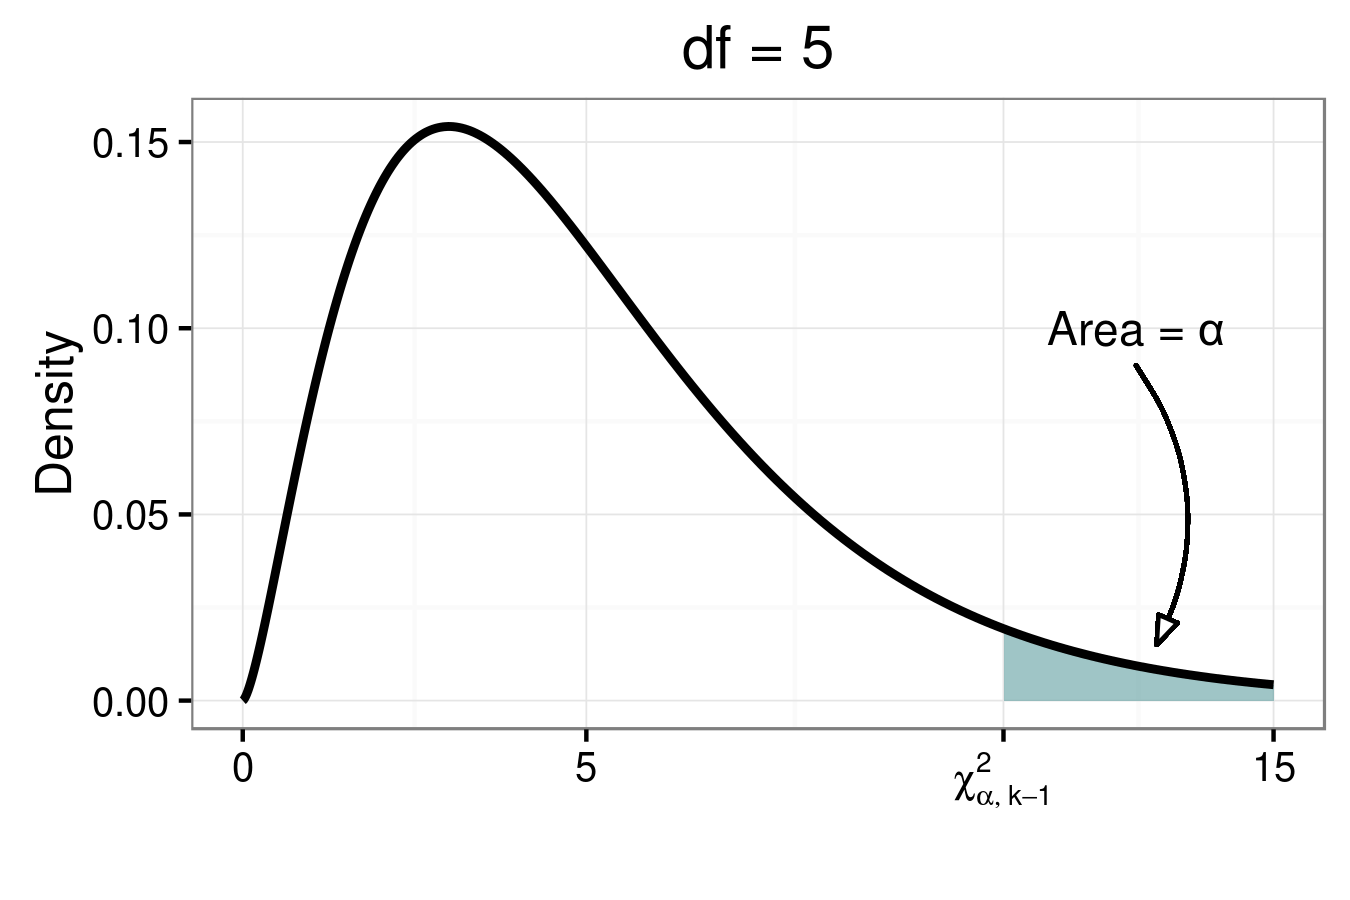
\includegraphics[width=4.5in]{../images/ch11_chi_square_crit}
\par}
\end{frame}



%%%%%%%%%%
\begin{frame}{Requirements for goodness-of-fit tests}
\begin{block}{}
\begin{itemize}
\item The sample is a simple random sample
\pause\item The sample data consists of frequency counts for each of the different categories
\pause\item For each class or category, the expected count is at least 5 
\end{itemize}
\end{block}
\end{frame}


%%%%%%%%%%
\begin{frame}{Uniform goodness-of-fit test, example}
\begin{exampleblock}{Example}
To determine if there is evidence is is not a die is ``fair", roll the die 40 times and perform a goodness-of-fit test on the results. \\
\medskip
A ``fair" die will have a uniform frequency distribution, so each result has a probability of 1/6 (16.67\%).
\medskip
\begin{itemize}
\pause\item $H_0:$ The frequency distribution of rolls fits a uniform distribution\\
$H_a:$ The frequency count of at least one result differs from the others

\pause\item Requirements: The expected count for each result is $E = \frac 1 6 \times 40 = 6.667 > 5$
\pause\item Find test statistic $\chi^2$, p-value and report decision
\end{itemize}
\end{exampleblock}
\end{frame}


%%%%%%%%%%
\begin{frame}<handout:0>{Group work}
\begin{block}{}
\large
\begin{itemize}
\item Complete question 2.
\end{itemize}
\end{block}
\end{frame}

%
% Section 10.3
%
\subsection{Tests for Independence}

%%%%%%%%%%
\begin{frame}{Contingency tables}
\begin{block}{}
Recall, a \bt{contingency table} is a two dimensional table (rows and columns) displaying frequency counts of classes or categories of two factors for a single sample.
\end{block}
\end{frame}

%%%%%%%%%%
\begin{frame}{Contingency tables, example}
\begin{exampleblock}{Example}
Recall the cancer screening example. A sample of 1000 randomly selected people where given a new screening test for a particular kind of of cancer. Each subject either has cancer or doesn't, and either tested positive or tested negative.\\
\medskip
{\centering
\begin{tabular}{c | c  c}
\multicolumn{1}{c}{} & \multicolumn{2}{c}{Test Result}\\
Diagnosis & Positive & Negative\\
\hline
Cancer & 74 & 13\\
No cancer & 26 & 887 \\
\end{tabular}
\par}
\smallskip

\end{exampleblock}
\end{frame}

%%%%%%%%%%
\begin{frame}{Contingency tables, example}
\begin{exampleblock}{Example}
Recall the example of the school distract attempting to reduce the rate of teen drivers who text or email. The school distract created an educational program that was attend by about half the students. Afterwards, a survey was taken of a sample of teen drivers. Each teen driver either attended the program or didn't, and either texted or emailed while driving or didn't.\\
\medskip
{\centering
\begin{tabular}{c | c  c}
\multicolumn{1}{c}{} & \multicolumn{2}{c}{Texted or emailed?}\\
Attended program? & Yes & No\\
\hline
Yes & 62 & 150\\
No & 59 & 114 \\
\end{tabular}
\par}
\smallskip

\end{exampleblock}
\end{frame}


%%%%%%%%%%
\begin{frame}{Independence in contingency tables}
\begin{block}{}
An important question that can be asked about data in contingency tables is whether the two factors are independent.\\
\pause\medskip
Factors are independent if the value of one factor does not impact the value of the other factor. In other words, if the probability of being in a category of one factor does not change depending on the category of the second factor, for all categories of both factors, then the factors are independent 
\end{block}
\end{frame}

%%%%%%%%%%
\begin{frame}{Independence in contingency tables}
\begin{exampleblock}{Example}
\begin{itemize}
\item For the cancer screening example, if the probability of testing positive is the same regardless of whether the subject has cancer or not, then the test results and cancer status are independent.

\pause\item For the teen driver example, if the probability of a teen driver texting or emailing is the same regardless of whether they attended the educational program or not, then texting or emailing and program attendance are independent.
\end{itemize}
\end{exampleblock}
\end{frame}

%%%%%%%%%%
\begin{frame}{Test for independence}
\begin{block}{}
A \bt{test for independence} is an hypothesis test which tests whether data contained in a contingency table represents two factors that are independent.
\begin{itemize}
\pause\item $H_0:$ The two factors are independent
\pause\item $H_a:$ The two factors are dependent\\
\pause\item Test statistic follows a $\chi^2$ (chi-squared) distribution with $(r-1) \times (c-1)$ degrees of freedom\\
\medskip
\eq{\chi^2 = \sum \frac {(O-E)^2}{E}}
\medskip
where
\begin{itemize}
\item $r$ is the number of rows and $c$ is the number of columns
\item $O$ is the observed count for each table cell, from sample
\item $E$ is the expected count for each table cell if the factors are independent
\end{itemize}
\end{itemize}
\end{block}
\end{frame}

%%%%%%%%%%
\begin{frame}{Expected counts}
\begin{block}{}
Like with goodness-of-fit tests, the expected count for each cell is the probability for that cell under the null hypothesis times the sample size.\\
\medskip
\eq{E = P(c) \times n}
\pause\medskip
Recall, if events are independent that the probability of both being true is the product of the probabilities of both.\\
\medskip
\eq{P(A \text{ and } B) = P(A) \times P(B)}

\pause\medskip
Thus, if $A$ is an event of one factor and $B$ is an event of the other factor, the expected count for the cell of $A$ and $B$ is\\
\medskip
\eq{E = P(A) \times P(B) \times n}
\medskip
\end{block}
\end{frame}

%%%%%%%%%%
\begin{frame}{Expected counts, cont.}
\begin{block}{}
The probability of an event of one factor is the marginal probability, the total count for the row or column divided by the total sample size.\\
\medskip
{\centering
\begin{tabular}{c | c  c | c}
\multicolumn{1}{c}{} & \multicolumn{2}{c}{Factor 2}\\
Factor 1 & B & $\sim$B & Total\\
\hline
A & \# (A and B) & \# (A and $\sim$B) & \# A\\
$\sim$A & \# ($\sim$A and B) & \# ($\sim$A and $\sim$B) & \# $\sim$A \\
\hline
Total & \# B & \# $\sim$B & n
\end{tabular}
\par}
\bigskip
\eq{P(A) = \frac {\# A}{n} \qquad P(B) = \frac {\# B} n}

\smallskip
\end{block}
\end{frame}

%%%%%%%%%%
\begin{frame}{Expected counts, cont.}
\begin{block}{}
Thus, the expected count for the cell of A and B is\\
\medskip
\eq{E_{A,B} = P(A) \times P(B) \times n = \frac {\# A} n \times \frac {\# B} n \times n}
\pause\bigskip
After some algebra, a simpler formula for expected count is\\
\medskip
\eq{E_{A,B}  = \frac{\# A \times \# B}{n}}
\medskip
\end{block}
\end{frame}

%%%%%%%%%%
\begin{frame}{Expected counts, example}
\begin{exampleblock}{Example}
\smallskip
{\centering
\begin{tabular}{c | c  c | c}
\multicolumn{1}{c}{} & \multicolumn{2}{c}{Test Result}\\
Diagnosis & Positive & Negative & Total\\
\hline
Cancer & 74 & 13 & 87\\
No cancer & 26 & 887 & 913 \\
\hline
Total & 100 & 900 & 1000
\end{tabular}
\par}
\bigskip
\begin{itemize}
\pause\item $\ds E_{+,\text{cancer}} = \frac {100 \times 87}{1000} = 8.7$
\pause\item $\ds E_{-,\text{cancer}} = \frac {900 \times 87}{1000} = 78.3$
\end{itemize}
\smallskip
\end{exampleblock}
\end{frame}

%%%%%%%%%%
\begin{frame}{Expected counts, example}
\begin{exampleblock}{Example}
\smallskip
{\centering
\begin{tabular}{c | c  c | c}
\multicolumn{1}{c}{} & \multicolumn{2}{c}{Test Result}\\
Diagnosis & Positive & Negative & Total\\
\hline
Cancer & 74 & 13 & 87\\
& (8.7) & (78.3)\\
No cancer & 26 & 887 & 913 \\
& (91.3) & (821.7)\\
\hline
Total & 100 & 900 & 1000
\end{tabular}
\par}
\smallskip
\end{exampleblock}
\end{frame}

%%%%%%%%%%
\begin{frame}{Decisions for tests for independence}
\begin{block}{}
Once a test statistic $\chi^2$ is found, the decision process for a test for independence is identical to the process for a goodness-of-fit test:
\begin{itemize}
\pause\item P-value: If the calculated p-value is less than the significance level ($p < \alpha$), then reject the null hypothesis.
\pause\item Critical value: If the calculated test statistic is greater than the critical value for the significance level and degrees of freedom ($\chi^2 > \chi^2_{\alpha, (r-1)(c-1)}$), then reject the null hypothesis.
\end{itemize}
\pause\medskip
For both methods, if conditions are not met to reject, fail to reject the null hypothesis.\\
\end{block}
\end{frame}


%%%%%%%%%%
\begin{frame}{Requirements for tests for independence}
\begin{block}{}
\begin{itemize}
\item The sample is a simple random sample
\pause\item The sample data consists of frequency counts for every cell of a contingency table
\pause\item For every cell, the expected count is at least 5 
\end{itemize}
\end{block}
\end{frame}


%%%%%%%%%%
\begin{frame}{Test for independence, example}
\begin{exampleblock}{Example}
Recall the cancer screening data:\\
\smallskip
{\centering
\begin{tabular}{c | c  c | c}
\multicolumn{1}{c}{} & \multicolumn{2}{c}{Test Result}\\
Diagnosis & Positive & Negative & Total\\
\hline
Cancer & 74 & 13 & 87\\
& (8.7) & (78.3)\\
No cancer & 26 & 887 & 913 \\
& (91.3) & (821.7)\\
\hline
Total & 100 & 900 & 1000
\end{tabular}
\par}
\bigskip
Test whether cancer diagnosis has an effect on the screening test result at $\alpha = 0.01$ level of significance.
\end{exampleblock}
\end{frame}

%%%%%%%%%%
\begin{frame}{Test for independence, example}
\begin{exampleblock}{Example}
\begin{itemize}
\pause\item $H_0:$ Test result and cancer diagnosis are independent\\
$H_a:$ Test result and cancer diagnosis are dependent (test result is associated with cancer diagnosis)
\pause\item Requirements: The smallest expected count, for cancer and positive test, is 8.7 which is larger than 5
\pause\item $\chi^2 = 596.47717$\\
$p < 0.0001 $
\pause\item $p < 0.0001 < 0.01 = \alpha$. Reject null hypothesis.
\pause\item There is evidence that test results and cancer diagnosis are associated.
\end{itemize}
\end{exampleblock}
\end{frame}

%%%%%%%%%%
\begin{frame}{Test for independence, example}
\begin{exampleblock}{Example}
Recall the teen driver data:\\
\medskip
{\centering
\begin{tabular}{c | c  c}
\multicolumn{1}{c}{} & \multicolumn{2}{c}{Texted or emailed?}\\
Attended program? & Yes & No\\
\hline
Yes & 62 & 150\\
No & 59 & 114 \\
\end{tabular}
\par}
\bigskip
Test whether texting or emailing while driving is associated with program attendance at $\alpha = 0.05$ level of significance.
\end{exampleblock}
\end{frame}

%%%%%%%%%%
\begin{frame}{Test for independence, example}
\begin{exampleblock}{Example}
\begin{itemize}
\pause\item $H_0:$ Texting or emailing and program attendance are independent\\
$H_a:$ Texting or emailing and program attendance are dependent (texting or emailing is associated with program attendance)
\pause\item Requirements: We don't have expected counts yet, but the sample size is in the hundreds and no outcome appears very unlikely. We can confirm when we have expected counts.
\pause\item $\chi^2 = 1.0435298$\\
$p = 0.307 $
\pause\item $p = 0.307 > 0.05 = \alpha$. Fail to reject null hypothesis.
\pause\item There is no evidence that texting or emailing while driving and program attendence are associated.
\end{itemize}
\end{exampleblock}
\end{frame}

%%%%%%%%%%
\begin{frame}{Test for independence vs. proportion test}
\begin{block}{}
We performed a proportion test with this data earlier. Testing the alternative hypothesis that the proportion of teen drivers who texted or emailed while driving was lower than for teens who attended the educational program than those who did not. \\
\begin{itemize}
\pause\item The results were $z = -1.02, \, p = 0.307$.\\
\pause\item The test for independence, while conducted as a one-sided test, is actually a two-sided test in that is does not distinguish between observed values that are lower or higher than expected values.\\
\pause\item Thus, the test for independence gave us identical results as the equivalent proportion test.
\end{itemize}
\end{block}
\end{frame}


%%%%%%%%%%
\begin{frame}<handout:0>{Group work}
\begin{block}{}
\large
\begin{itemize}
\item Complete questions 3.
\end{itemize}
\end{block}
\end{frame}


\end{document}